\section{Discussion}\label{sec:bool_discussion}
When inspecting figure \ref{fig:Searchtimebool1} and figure \ref{fig:Searchtimebool7} it is important to keep in mind that the measurement includes both evaluating the whole Boolean query tree as well as decoding the resulting encoded article list. 

To summarise and compare the indices, the number of computational steps of each Boolean operation, when evaluating a Boolean query of depth 1 and decoding the resulting article list, have been gathered in table \ref{tab:Booleanruntimes1}. The run-time complexities of the operations are gathered in table \ref{tab:BooleanruntimesO}. The purpose of table \ref{tab:Booleanruntimes1} is to estimate the number of steps required to perform the operation and thereby compare the expected coefficient of the linear growths. The contents of the tables are detailed in the following. 

%An article list $A_n$ is upper bounded by $O(a)$. This means that all operations in table \ref{tab:Booleanruntimes1} has the time complexity $O(a)$ except for the AND operation for Index8.2 and 8.3, which is bounded by $O(min(|A_i| + |A_j|, log(|A_i|)\cdot |A_j|))$, and $\lceil \frac{a}{64} \rceil$ and $a$ which has the tight bound $\Theta(a)$. 

\begin{table}[H]
\begin{tabular}{l|lllp{2cm}}
    Index & AND & OR & INVERSION & Decoding of article list\\
\hline
7.0 &  $\lceil \frac{a}{64} \rceil$   &  $\lceil \frac{a}{64} \rceil$  &  $\lceil \frac{a}{64} \rceil$ & $a$         \\
8.0 &  $|A_i| + |A_j|$   &  $|A_i| +|A_j|$  &  $|A_i|$  & $|A_{result}|$       \\
8.1 &  $|A_i| + |A_j|$   &  $|A_i| + |A_j|$  &  $|A_i|$  & $|A_{result}|$         \\
8.2 &  $\min(|A_i| + |A_j|, \log(|A_i|)\cdot |A_j|)$   &  $|A_i| + |A_j|$  &  $|A_i|$  & $|A_{result}|$    \\
8.3 &  $\min(|A_i| + |A_j|, \log(|A_i|)\cdot |A_j|)$   &  $|A_i| + |A_j|$  &  $|A_i|$  & $|A_{result}|$     \\
8.4 &  $|A_i| + |A_j| + \lceil \frac{a}{64} \rceil$   &   $|A_i| + |A_j| + \lceil \frac{a}{64} \rceil$   &  $|A_i| + \lceil \frac{a}{64} \rceil$   & $a$
\end{tabular}
\caption{For each Index and operation, the number of computational steps is estimated. As in $O$-notation, these estimates are simply proportionality factors and thus have unknown constants associated. }
\label{tab:Booleanruntimes1}
\end{table}

\begin{table}[H]
\begin{tabular}{l|lllp{2cm}}
    Index & AND & OR & INVERSION & Decoding of article list\\
\hline
7.0 &  $\Theta(a)$   &  $\Theta(a)$  &  $\Theta(a)$ & $\Theta(a)$         \\
8.0 &  $O(a)$   &  $O(a)$  &  $O(a)$  & $O(a)$       \\
8.1 &  $O(a)$   &  $O(a)$  &  $O(a)$  & $O(a)$         \\
8.2 &  $O(\min(|A_i| + |A_j|, \log(|A_i|)\cdot |A_j|))$   &  $O(a)$  &  $O(a)$  & $O(a)$    \\
8.3 &  $O(\min(|A_i| + |A_j|, \log(|A_i|)\cdot |A_j|))$   &  $O(a)$  &  $O(a)$  & $O(a)$     \\
8.4 &  $\Theta(a)$   &   $\Theta(a)$   &  $\Theta(a)$   & $\Theta(a)$
\end{tabular}
\caption{Runtime complexities for each Boolean operation for each Boolean index for a query of depth 1. }
\label{tab:BooleanruntimesO}
\end{table}

\subsection{Comparing the two pointer system to bit operations on complete Boolean query trees}

In figure \ref{fig:Searchtimebool1} it is seen that Index7.0 in general slightly faster than the other indices. All Boolean operations of 7.0 do however have a time complexity of $\Theta(a)$. Index7.0 might therefore perform more steps than the other indices but because it utilises the bit wise operations, which are performed very fast, it has very good constants compared to the other indices. This does however come at the cost of Index7 being the most expensive index in terms of space complexity, as it stores the article list using $\Theta(a)$ bits. 

Index8.4 does also use fast bit-wise Boolean operations, but before doing so it needs to convert the article list, to a bit vector article list. When comparing Index8.0 and 8.4 on queries of depth 1 in table \ref{tab:Booleanruntimes1} it is clear to see that 8.0 should be better, as it excludes the $\lceil \frac{a}{64} \rceil$ term. Creating the bit-wise article lists costs the same as performing the AND operation of Index8.0 itself. Furthermore the decoding of the article list of Index8.0 upper bounded by $O(a)$ whereas decoding of the article list of Index8.4 is tightly bounded by $\Theta(a)$, as the decoding of the article list of Index8.4 always evaluates $a$ bits. Index8.4 does therefore not perform greatly, compared to the other indices, when the depth only is 1, which corresponds to the tendency observed in figure \ref{fig:Searchtimebool1}.

However, when the depth of the search query increases, Index7.0 and 8.4 is expected to be faster than any of the other indices. This tendency is represented in figure \ref{fig:Searchtimebool7}. Table \ref{tab:Booleanruntimesd} shows an estimate for the number of computational steps needed to evaluate a tree of depth $d$, consisting of only either the AND, the OR or the INVERSION operator.

\begin{table}[H]
\begin{tabular}{l|lll}
Index 
& AND                           
& OR                             
& INVERSION \\         
\hline
7.0 
&  $\lceil \frac{a}{64} \rceil \cdot (2^d-1)$   
&  $\lceil \frac{a}{64} \rceil \cdot (2^d-1)$  
&  $\lceil \frac{a}{64} \rceil \cdot d$         \\
8.0 
&  $\sum_{n=1}^{2^{d+1}-2}(|A_n|)$        
&  $\sum_{n=1}^{2^{d+1}-2}(|A_n|)$       
&  $\sum_{n=1}^{d}(|A_n|)$             \\
8.4 
&  $\sum_{n=1}^{2^{d}}(|A_n|) + (2^{d}-1) \cdot \lceil \frac{a}{64} \rceil$   
&  $\sum_{n=1}^{2^{d}}(|A_n|) + (2^{d}-1) \cdot \lceil \frac{a}{64} \rceil$   
&  $A_1 + d \cdot \lceil \frac{a}{64} \rceil$   
\end{tabular}
\caption{For each Boolean operation and index, an estimate for the number of computational steps needed to evaluate a tree of depth $d$, consisting of only that operation is given. }
\label{tab:Booleanruntimesd}
\end{table}

A query tree of depth $d$ consisting of either AND operators or OR operators is a complete binary tree. The depth $d$ of the tree is defined as the maximum number of edges from the root to a leaf. There are thereby $2^{d+1}-1$ nodes in total, where $2^d$ of the nodes are leaves and $2^d-1$ nodes are parent nodes. To evaluate the query tree using Index8.0, $2^d-1$ Boolean operations must be performed - one for each parent. In the complete binary tree, the article lists of the leaves and the resulting article evaluated by the Boolean operators of the tree are denoted $A_n$ for $n=1..2^d$. A visual illustration of the order is shown in figure \ref{fig:An}. 

\begin{figure}[bh!]
    \centering
    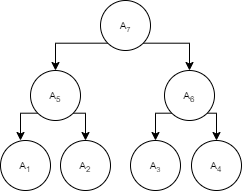
\includegraphics[width=.5\textwidth]{LaTeX/Figures/An.drawio.png}
    \caption{Visual illustration of how the $A_n$ article list are numbered for a tree of height 2}
    \label{fig:An}
\end{figure}


Performing one Boolean operation in 8.0 takes time proportional to the length of the article lists of the children of the node. Thereby $\sum_{n=1}^{2^{d+1}-2}(|A_n|)$ in total - every node expect the root. Whereas 8.4 needs to convert all article lists of leaves into bit vectors taking $\sum_{n=1}^{2^{d}}(|A_n|)$ steps and hereafter evaluate $2^d-1$ Boolean operations each taking $\lceil \frac{a}{64} \rceil$ time. The difference between 8.0 and 8.4, therefore, comes down to 

\begin{equation} \label{eq1}
\begin{split}
 AND_{8.0} - AND_{8.4} & = \left[\sum_{n=1}^{2^{d+1}-2}(|A_n|)\right] - \left[\left(\sum_{n=1}^{2^{d}}(|A_n|)\right) + (2^{d}-1) \cdot \left\lceil \frac{a}{64} \right\rceil\right] \\
 & = \left(\sum_{n=2^d}^{2^{d+1}-2}(|A_n|)\right) - \left((2^{d}-1) \cdot \left\lceil \frac{a}{64} \right\rceil\right)
\end{split}
\end{equation}

The first term of the result represents the steps needed for Index8.0 to evaluate the second half of the query tree (all the nodes in the tree with a height of $\leq d-1$). The second term represents steps needed for Index8.4 to evaluate all parent nodes after the leaves have been converted to bit vectors.
$\sum_{n=2^d}^{2^{d+1}-2}(|A_n|)$ is upper bounded by $O(a)$ whereas $(2^{d}-1) \cdot \lceil \frac{a}{64} \rceil$ is tightly bounded by $\Theta(a)$. Index8.4 is therefore expected to perform more steps than Index8.0 for large $a$. Index8.4 is however still expected to be faster as it utilises bit wise Boolean operation, which can be performed super fast, compared to Index8.0, which compares two characters, adds one of them to a result list, and hereafter moves a pointer. This is the same tendency as seen in figure \ref{fig:Searchtimebool1}, where Index7.0 where the faster search time. The performance of Index8.0 compared to Index8.4 is however greatly dependent on the expected length of the article list in the second half of the query tree. A short article list compared to $\lceil \frac{a}{64} \rceil$ will give Index8.0 an advantage that at some point might outperform the bit-wise operations of Index8.4. The length of the article list in the second half of the query tree is however greatly dependent on the Boolean operators in the tree. 

The AND operation returns the intersection, $A_{result}$, of the article list of the two children, $A_i$ and $A_j$. This means that $|A_{result}|\leq min(|A_i|,|A_j|)$. The AND operation using the two pointer system is therefore expected to run faster at nodes higher in a tree only constructed by AND operations as the incoming article lists are expected to be shortened. A Boolean query tree consisting of exclusively AND operator will appear in the chapter discussing Full Text indexing - the bit wise method of Index7.0 and 8.4 is therefore not chosen to calculate this intersection.

The exact opposite is expected for a tree only consisting of OR nodes as OR nodes calculate the union of two article lists making $|A_{result}|\geq \max(|A_i|,|A_j|)$. This is a great disadvantage for 8.0 and makes 8.4 much better at evaluating Boolean trees, with a large $d$, only consisting of OR operators. This exact type of tree will appear in the chapter Prefix search.

Calculating the distribution of length of the resulting article list that the Boolean operators return in a tree of mixed Boolean operators, given the distribution of lengths of the articles list for each word, is a non-trivial probability assignment, that we haven't analysed nor simulated. However, when simply looking at the length of the article list for each word, it is seen that the majority of words have short article lists. This tendency can be seen in Figure \ref{fig:Articlelength20}. Histograms for the other file sizes can be found in the appendix.

\begin{figure}[ht!]
    \centering
    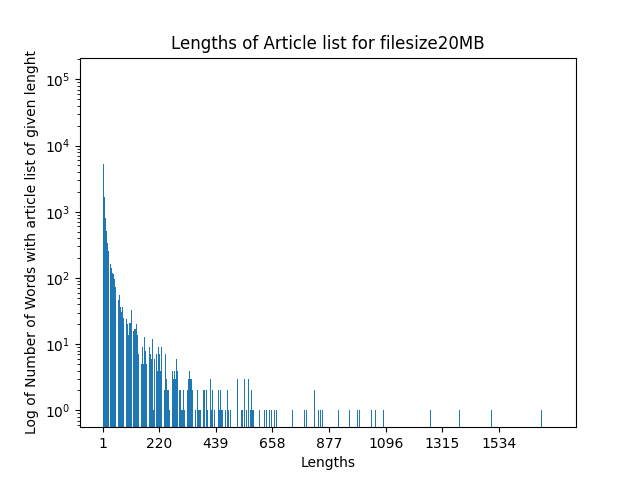
\includegraphics[width=.7\textwidth]{LaTeX/Pictures/Results/ArticleLengthg20MB.png}
    \caption{Histogram over the frequency of word with article list of a given length for filesize 20 MB}
    \label{fig:Articlelength20}
\end{figure}

It is an advantage for Index8.4 when the Mean length of the article list is high relative to $\lceil \frac{a}{64} \rceil$. Table \ref{tab:MeanArticlelengh_a26} however shows that this not is the case when looking at larger file sizes. This tendency is of course dependent on the contents of the database. This shows that the article bit vector that Index8.4 calculates at some point will be too expensive to compute. When looking at figure \ref{fig:Searchtimebool7} where the indices were tested on trees of mixed Boolean operators, Index8.4 is however still superior to Index8.0, even though Index8.4 is expected to perform more steps. This is the same tendency seen in figure \ref{fig:Searchtimebool1} where 7.0 is superior, despite its poorer runtime complexity. Index8.4 and 7.0 are both predicted to perform more steps but as they utilise the fast bit operations they can still manage to outperform the slower but fewer two-pointer system steps for Index8.0. 

\begin{table}[H]
\centering
\begin{tabular}{l|lllllllll}
 Filesize (MB)                           & 0.1 & 1     & 2      & 5      & 10 & 20     & 50     & 100 & 200 \\
 \hline 
Mean length of article list &  1.22   & 2.46     & 3.13      & 4.23      & 5.48      &  6.85     &  9.54    &  12.06      &  15.36      \\
  $\lceil \frac{a}{64} \rceil$                          &  1      & 1        & 2         &  6        & 14      &  28       &  66     & 129     &  282    
\end{tabular}
\caption{Mean article list length for each file size}
\label{tab:MeanArticlelengh_a26}
\end{table}

Even though Index7.0 and 8.4 performs better than the other indices as seen in figure \ref{fig:Searchtimebool7}, Index7.0 and 8.4 would rarely be chosen over the other indices in a real-life setting with larger databases. This is due to the fact that they are too expensive in both memory and search time when $a$ is large. Index7.0 uses $\Theta(a\cdot u)$ space to simply store the index. Even though 8.4 only uses $\Theta(u)$ space to store the index, the extra space used when searching will at some point become too expensive as a $O(a)$ bit wise article list needs to be created per word in the search query.

\subsection{Commenting Index8.1, 8.2 and 8.3}

Index8.0, 8.1, 8.2 and 8.3 all perform similarly. This tendency does not change when the depth of the query is increased. This may indicate that the small changes in using De-Morgans law or binary search or both are not visibly different. The randomly generated queries may not generate enough cases where the additional evaluation features are helpful. The time won may therefore not outweigh the extra time it takes to check if the evaluation feature can be used. 

The set up of the timing may not justify the potential of Index8.1 and 8.2. To show the full potential of these indices we would in hindsight have liked to create more benchmarking timing specifically designed for these. E.g. timing 1000 examples of evaluating a query on the form $!A \vee ! B$ and $!A \wedge ! B$  compared to $!(A \wedge B)$ and $!(A \vee B)$. Using De-Morgans law is theoretically beneficial as it omits one inversion, which is the most expensive Boolean operation. Performing a test with a focus on this would therefore be interesting to see how much time is won in practice, and if it would be possible to map the change to performing precisely one inversion less.

It is however worth pointing out that De-Morgans law rarely occurs in either naturally generated search queries or other practical uses where a Boolean query tree might appear. This means that there rarely is any time to win using this method. Checking to see when the method can be used therefore seems inconvenient, as omitting one inversion is negligible when looking at a lot of queries as in figure \ref{fig:Searchtimebool1}.

To justify 8.2, queries where the binary search approach is helpful could be constructed. These queries could then be evaluated by both Index8.2 and Index8.0 and compared. In theory, 8.2 should perform better once again. Furthermore, it would be possible to determine the constants $c_1, c_2$ in $c_1\cdot|A_0| \cdot \log_2(|A_1|) < c_2\cdot (|A_0| +  |A_1|)$ to make Index8.2 even better at deciding when to use the binary search approach and when not to.

As none of the indices filter out any stop words, such as "a", "the" and "that", other than grammatical characters, the binary search feature could potentially be very useful. This is because stop words occur in almost all articles, whereas most other words only occur in a few articles. Even though 8.4 performs much better than Index8.2 at the file sizes tested in these plots, generating the bit-wise article list will at some point become too expensive when $a$ grows. Therefore 8.2 would be interesting to develop further.
